% Phase 4 (Héctor Armenteros): Probabilities and System Size N = 100 + M (Part 2 a–d).
% All numerical values generated by src/thermodynamics.py (python -m src.thermodynamics).

\subsection{Probabilities and Macrostate Intervals for \texorpdfstring{$N = 100 + M$}{N = 100 + M}}

\paragraph{System size.} $M$ is the harmonic average of the last two digits of the members' NIAs, $69$ (Guillermo), $22$ (Andr\'es), $09$ (H\'ector, taken as $9$) and $45$ (Carlos):
\begin{equation}
    M = \frac{4}{\frac{1}{69} + \frac{1}{22} + \frac{1}{9} + \frac{1}{45}} = \frac{4}{0.193281} = 20.6953 \;\to\; M = 21, \qquad N = 100 + M = 121 \text{ coins},
\end{equation}
rounding to the nearest integer. Since $N$ is odd, $N/2 = 60.5$ is not a macrostate: the distribution has two degenerate peaks, $k = 60$ and $k = 61$, with $\Omega(121, 60) = \Omega(121, 61)$. Probabilities are computed in log space, $P(N,k) = \exp[\ln\Omega(N,k) - N\ln 2]$, with \texttt{ln\_omega} (Section~\ref{sec:microstates}), and checked in \texttt{tests/test\_thermodynamics.py}. Figure~\ref{fig:probabilities} shows the distribution and the intervals below; Table~\ref{tab:largeN} collects the answers.

\paragraph{(a) $k = 30$ heads.} $P(121, 30) = 8.490094 \times 10^{-9}$. This state lies $5.55\sigma$ from the mean ($\sigma = \sqrt{N}/2 = 5.50$ coins): less than 1 in 100 million, showing how fast the binomial tail vanishes.

\paragraph{(b) Most probable macrostate ($k = N/2$).} $P(121, 60) = P(121, 61) = 0.072089$ ($7.21\,\%$), with $\Omega(121, 60) \approx 1.916167 \times 10^{35}$ microstates each; the system is in either of them with probability $P(60) + P(61) = 0.144179$ ($14.42\,\%$).

\paragraph{(c) Heads in $[N/2 - 10, N/2 + 10]$.} The interval $[50.5, 70.5]$ covers the 20 macrostates $k \in [51, 70]$:
\begin{equation}
    \Delta P_{\text{heads}} = \sum_{k=51}^{70} P(121, k) = 0.931406 \quad (93.14\,\%).
\end{equation}
Centred on the integer mode $k = 60$, the 21 macrostates in $[50, 70]$ give $\Delta P = 0.943177$ ($94.32\,\%$), and $[50, 71]$ (22 states) gives $0.954948$ ($95.49\,\%$). A band of only $16.4\,\%$ of the macrostates holds over $93\,\%$ of the probability.

\paragraph{(d) Tails in $[N/2 - 20, N/2 + 20]$.} With $t = N - k$ tails and $p = q = 1/2$, the distribution is invariant under heads $\leftrightarrow$ tails, $P_{\text{tails}}(N, t) = P_{\text{heads}}(N, t)$. The interval $t \in [40.5, 80.5]$, i.e.\ $t \in [41, 80]$, is $41 \le k \le 80$ in heads:
\begin{equation}
    \Delta P_{\text{tails}} = \sum_{t=41}^{80} P(121, t) = 0.999756 \quad (99.9756\,\%).
\end{equation}
Around the integer mode, $[40, 80]$ gives $0.999820$ ($99.982\,\%$). The window is $\pm 20/\sigma \approx \pm 3.64$ standard deviations, so the system falls outside it less than $0.025\,\%$ of the time.

\begin{figure}[htbp]\centering
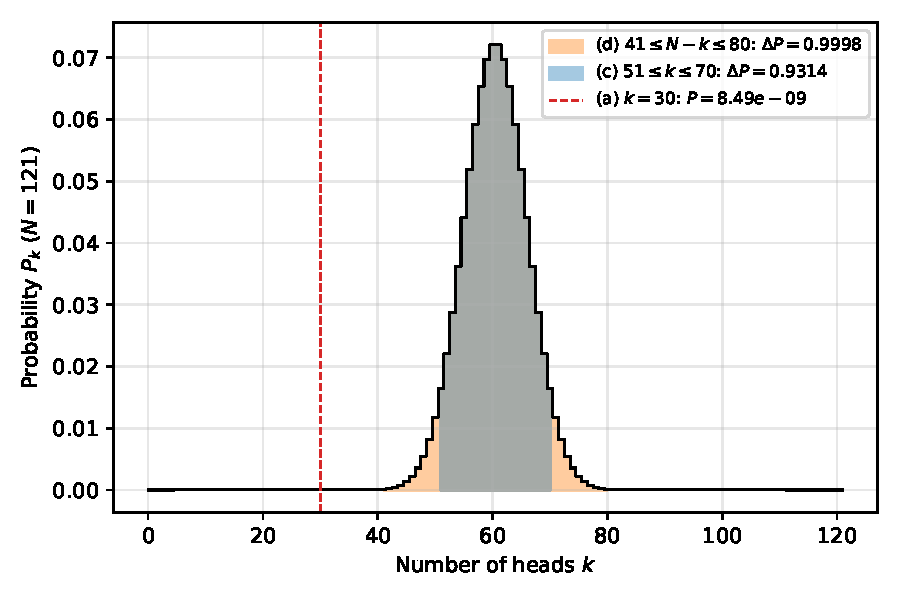
\includegraphics[width=0.55\textwidth]{figures/probability_distribution.pdf}
\caption{Probability $P(121, k)$ against the number of heads $k$ for $N = 121$. Shaded: the intervals of 2c ($\pm 10$ heads, $\Delta P = 0.9314$, blue) and 2d ($\pm 20$ tails, $\Delta P = 0.9998$, orange); dashed red line: $k = 30$ of 2a ($P = 8.49 \times 10^{-9}$).}\label{fig:probabilities}
\end{figure}
